\documentclass[pdf]{beamer}
\mode<presentation>{} 

\usepackage{hyperref}
\usepackage{pgf}
\usepackage{tikz}
\usetikzlibrary{trees}
\usetikzlibrary{arrows,automata}
\usetikzlibrary{automata,positioning}
\usetikzlibrary{shapes}
\usepackage{tikz-qtree,tikz-qtree-compat}
\usepackage{mathtools,enumerate,amssymb}
\usepackage[utf8]{inputenc}
\usepackage[T1]{fontenc}
\usepackage{graphicx}
\usepackage{tabularx}

\title{Criptosisteme}
\subtitle{Securitate informatică}
\AtBeginSection[]{}

\setbeamertemplate{sidebar right}{}
\setbeamertemplate{footline}{%
\hfill\usebeamertemplate***{navigation symbols}
\hspace{1cm}\insertframenumber{}/\inserttotalframenumber}

\begin{document}

\begin{frame}
	\titlepage
	
\begin{flushright}
Mihai-Lica Pura\\
\end{flushright}

\end{frame}



\begin{frame}{Cuprins}
\begin{itemize}
\item
Criptosisteme
\item
Funcții hash criptografice
\item
Message Authentication Codes
\item
Criptografia cu chei simetrice
\item
Criptografia cu chei asimetrice
\item
Criptografia hibridă
\item
Key agreement
\item
Standardele criptografiei cu chei publice
\end{itemize}
\end{frame}



\begin{frame}{Security services, security protocols, security mechanisms, cryptosystems}
\begin{itemize}
\item
\textbf{Security services} are implemented through security protocols

\item
A typical security protocol provides one or more security services

\item
Security protocols are implemented using one or more \textbf{security mechanisms}

\item
Security mechanisms are implemented using \textbf{algorithms}

\item
\textbf{Cryptosystems} are one particular type of suits of algorithms used to implement security mechanisms

\end{itemize}
\end{frame}



\begin{frame}{Security services, security protocols, security mechanisms, cryptosystems}

\begin{figure}[t]
\centering
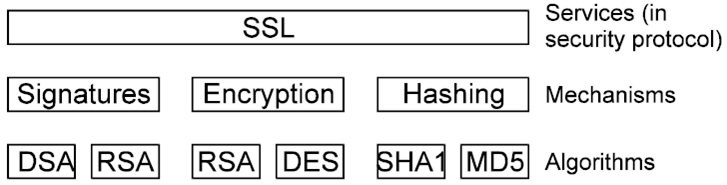
\includegraphics[scale=0.5]{Images/SSSM}
\end{figure}

\end{frame}



\begin{frame}{Cryptosystems}
\begin{itemize}
\item
\textbf{cryptosystem} - a suite of cryptographic algorithms needed to implement a particular security service

\item
typically, a cryptosystem consists of algorithms for key generation, encryption, and decryption

\item
\textbf{cipher (or cypher)} - an algorithm for performing encryption or decryption

\begin{itemize}
\item
the cipher depends on a piece of auxiliary information, called \textbf{key}

\item
without knowledge of the key, it should be unfeasible to decrypt the resulting ciphertext into readable plaintext
\end{itemize}

\end{itemize}
\end{frame}



\begin{frame}{Cryptosystems}
\textbf{Ciphers classification:}
\begin{itemize}
\item
\textbf{symmetric key} algorithms - the same key is used for both encryption and decryption 
\item
\textbf{asymmetric key} algorithms - a different key is used for each 
\end{itemize}

\begin{itemize}
\item
\textbf{block ciphers} - work on blocks of symbols usually of a fixed size 

\item
\textbf{stream ciphers} - work on a continuous stream of symbols

\end{itemize}
\end{frame}



\begin{frame}{Cryptosystems for security mechanism}
\begin{itemize}
\item
\textbf{Cryptographic hash algorithms}

- used to provide integrity protection

- can provide authentication (using Message Authentication Codes - MACs)

\item
\textbf{Encryption}

- used to provide confidentiality

- can provide authentication and integrity protection

\item
\textbf{Digital signatures} 

- used to provide authentication, integrity protection, and non-repudiation

\end{itemize}
\end{frame}



\begin{frame}{Cryptographic Hash Functions}
\begin{itemize}
\item
are designed to take a string of any length as input and produce a fixed-length hash value

\item
are used to assure integrity and authentication

\item

- SHA1(securitate informatica) = 7ea5a44914425634e7ad6153bbcc4548fd98b51b

- SHA256(securitate informatica) = bdbc3602d0a30e171ba3fa1f839701693303de05cf347cf050bcdf27428a07a9

- SHA256(compilatoare) = 
05ace8a1c5faf8fbc2c72cffee83b15131a09292b69f9eefa6e5a4f2ce03476d

\end{itemize}
\end{frame}



\begin{frame}{Cryptographic Hash Functions}
\textbf{Requirements for a Cryptographic Hash Function:}
\begin{itemize}
\item
H can be applied to a block of data of any size

\item
H produces a fixed-length output

\item
H(x) is relatively easy to compute for any given x, making both hardware and software implementations practical

\item
For any given value h, it is computationally infeasible to find x such that H(x) = h (\textbf{one-way property})

\item
For any given block x, it is computationally infeasible to find $y \neq x$ such that H(y) = H(x) (\textbf{weak collision resistance})

\item
It is computationally infeasible to find any pair (x, y) such that H(x) = H(y) (\textbf{strong collision resistance})

\end{itemize}
\end{frame}



\begin{frame}{Cryptographic Hash Functions}
\textbf{Use:}
\begin{itemize}
\item
verifying the integrity of files or messages (MAC)

\item
password protection and verification (with care)

\item
in the generation of pseudorandom bits, or to derive new keys or passwords from a single, secure key or password

\item
widely used as file or Object identifier in e.g. Git, Mercurial and some p2p-file-sharing networks

\end{itemize}
\end{frame}



\begin{frame}{Cryptographic Hash Functions}
\textbf{General purpose Hash functions:}
\begin{itemize}
\item
\textbf{MD4(128)} - not recommended anymore

\item
\textbf{MD5(128)} - not recommended anymore

\item
\textbf{SHA-1 (160)} - not recommended anymore

\item
\textbf{SHA-2 (224, 256)}

- is state of the art and is recommended function to be used in e.g. X.509 Certificates

\item
\textbf{SHA-3 (224, 256, 384, 512)}

- is build for future and very new and is not broadly supported at the moment

\end{itemize}
\end{frame}



\begin{frame}{Cryptographic Hash Functions}
\textbf{SHA parameters}
\begin{figure}[t]
\centering
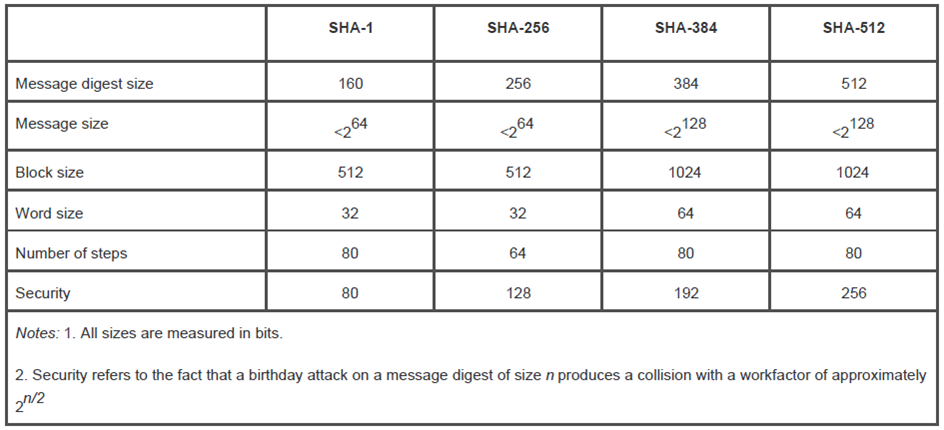
\includegraphics[scale=0.45]{Images/sha}
\end{figure}
\end{frame}



\begin{frame}{Cryptographic Hash Functions}
\textbf{Hash and Passwords:}
\begin{itemize}
\item
general purpose hash functions are sometimes used for password hashing

BUT 

\item
they are to "too fast" on modern hardware, which makes them weak against brute-force attack

SO

\item
just \textbf{DON'T use general purpose hashing algorithms for password hashing}

\item
instead use one of the \textbf{hash functions designed for password protection}

\begin{itemize}
\item
PBKDF2 
\item
bcrypt, scrypt
\item
\textbf{Argon2} - the winner of the Password Hashing Competition in July 2015
\end{itemize}

\end{itemize}
\end{frame}



\begin{frame}{Cryptographic Hash Functions}
\textbf{Argon2:}
\begin{itemize}
\item
designed by Alex Biryukov, \textbf{Daniel Dinu (Military Technical Academy graduate)}, and Dmitry Khovratovich from the University of Luxembourg

\item
source code: 

\url{https://github.com/p-h-c/phc-winner-argon2}

\end{itemize}
\end{frame}



\begin{frame}{Message Authentication Codes}

\begin{itemize}
\item
objectives:  
\begin{itemize}
\item
data integrity
\item
data authentication
\end{itemize}

\item
does NOT provide non-repudiation of data origin

\item
similar to hash, but adds a key/password to the hash:
\begin{itemize}
\item
MAC = C(K, M)
\end{itemize}

\item
only the password holder(s) can generate/verify the MAC

\item
a MAC function is similar to encryption - one difference is that the MAC algorithm needs to be irreversible

\item
does not allow a distinction to be made between the parties sharing the key/password

\item
(crypto) algorithms: AES-MAC, DES-MAC, HMAC (SHA1/SHA2/SHA3), …

\end{itemize}
\end{frame}



\begin{frame}{Message Authentication Codes}
\begin{figure}[t]
\centering
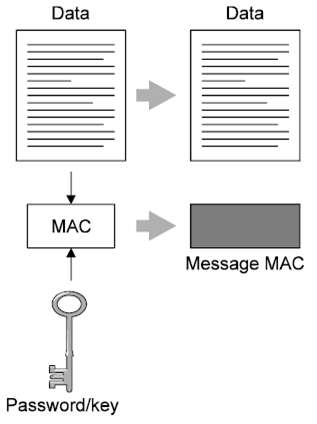
\includegraphics[scale=0.65]{Images/MAC}
\end{figure}
\end{frame}



\begin{frame}{Message Authentication Codes}
\textbf{Message authentication}
\begin{figure}[t]
\centering
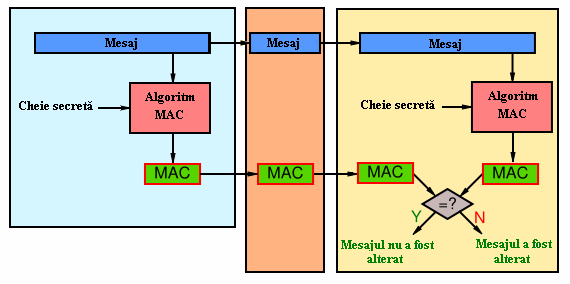
\includegraphics[scale=0.9]{Images/MAC2}
\end{figure}
\end{frame}



\begin{frame}{Message Authentication Codes}
\begin{figure}[t]
\centering
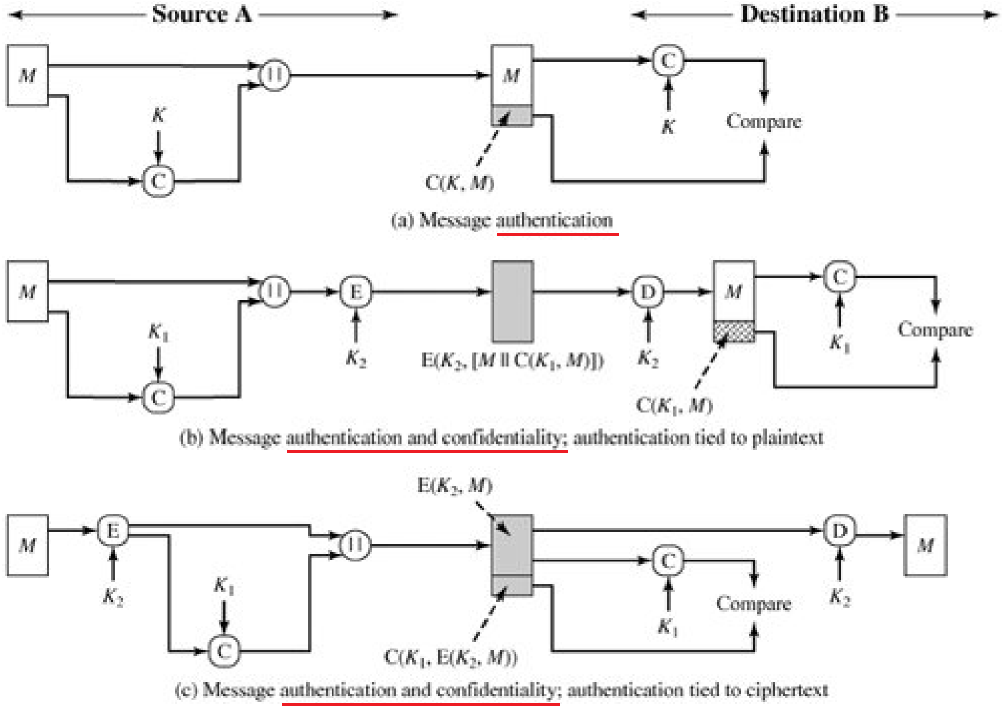
\includegraphics[scale=0.53]{Images/macuse}
\end{figure}
\end{frame}



\begin{frame}{Message Authentication Codes}
\begin{itemize}
\item
\textbf{Hash Message Authentication Code (HMAC)}
\begin{itemize}
\item
RFC 2104 is from 1997
\item
just a specific type of MAC that is based on hash functions
\item
any cryptographic hash function may be used in the calculation of an HMAC
\item
cryptographic strength of the HMAC depends upon:
\begin{itemize}
\item
the cryptographic strength of the underlying hash function
\item
the size of its hash output
\item
the size and quality of the key
\end{itemize}
\end{itemize}

\item
\textbf{Cipher-based Message Authentication Code (CMAC)}
\begin{itemize}
\item
CMAC or CMAC-AES (RFC 4493 from 2006)
\item
MAC algorithm for block ciphers
\item
CMAC can be calculated faster if target platform utilizes hardware optimization for block ciphers (e.g. dedicated AES opcodes)
\end{itemize}
\end{itemize}
\end{frame}



\begin{frame}{Message Authentication Codes}
\begin{itemize}
\item
\textbf{Universal Hashing MAC (UMAC)}
\begin{itemize}
\item
RFC 4418 from 2006
\item
MAC based on universal hashing
\item
the resulting digest is then encrypted to hide the identity of the used hash function for additional security
\item
UMAC has provable cryptographic strength and is usually a lot less computationally intensive than other MACs
\item
UMAC's design is optimized for 32-bit architectures
\item
VMAC - a closely related variant of UMAC that is optimized for 64-bit architectures
\end{itemize}

\item
\textbf{Poly1305}
\begin{itemize}
\item
Google has selected Poly1305 along with symmetric cipher ChaCha20 as a replacement for RC4 in TLS/SSL
\end{itemize}
\end{itemize}
\end{frame}



\begin{frame}{Symmetric-key cryptography}
\begin{itemize}
\item
objective:
\begin{itemize}
\item
data confidentiality (data privacy)
\end{itemize}

\item
\textbf{stream ciphers:}
\begin{itemize}
\item
RC4 - meanwhile considered insecure!
\item
Salsa20 - very effcient and secure. ChaCha variant was selected as a replacement for RC4 in OpenSSL.
\item
SEAL - one of the fastest stream ciphers
\item
A5/1,A5/2 - are used in GSM and considered weak and insecure! 
\item
SNOW 3G - synchronous stream cipher
\item
HC-256 - gains popularity
\item
Rabbit - gains popularity
\end{itemize}

\end{itemize}
\end{frame}



\begin{frame}{Symmetric-key cryptography}
\begin{itemize}
\item
\textbf{block ciphers:}
\begin{itemize}
\item
DES
\item
AES
\item
IDEA (1990, International Data Encryption Algorithm) - used in PGP
\item
Blowfish (1993, Bruce Schneier)
\item
Twofish - used by Microsoft
\item
CAST-128, CAST-256 (Carlisle M. Adams)
\item
Serpent (Ross Anderson, Eli Biham und Lars Knudsen)
\item
RC5
\end{itemize}

\item
usages:
\begin{itemize}
\item
data encryption
\item
MACs
\end{itemize}

\end{itemize}
\end{frame}



\begin{frame}{Symmetric-key cryptography}
\begin{figure}[t]
\centering
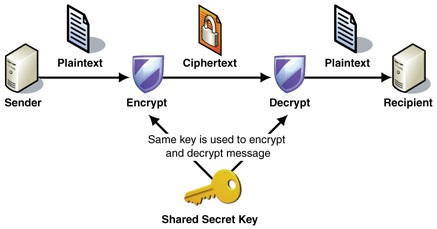
\includegraphics[scale=1]{Images/IC168364}
\end{figure}
\end{frame}



\begin{frame}{Symmetric-key cryptography}
\begin{itemize}
\item
plaintext is encrypted into ciphertext on the sender side 

\item
the same key (key copy) is used to decrypt the ciphertext to plaintex on the recipient side

\item
as long as both sender and recipient know the secret key, they can encrypt and decrypt all messages that use this key

\item
\textbf{drawback}:  both parties must know the same secret key - sharing of key must be done in a secure way


\end{itemize}
\end{frame}



\begin{frame}{Symmetric-key cryptography}
\begin{itemize}
\item
uses a secret shared key

\item
the problem of communicating a large message in secret is reduced to the problem of communicating a small key in secret

\item
the new \textbf{Big Issue}: management (sharing) of the secret key

\end{itemize}
\end{frame}



\begin{frame}{Symmetric-key cryptography}
\begin{figure}[t]
\centering
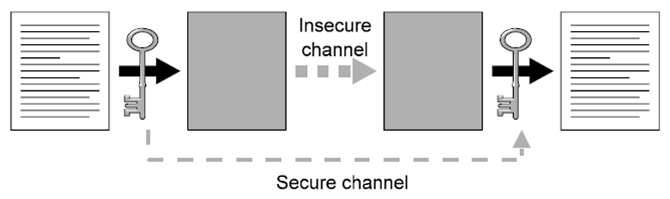
\includegraphics[scale=0.5]{Images/sym}
\end{figure}
\end{frame}



\begin{frame}{Asymmetric-key cryptography}
\begin{itemize}
\item
objective:  
\begin{itemize}
\item
data confidentiality (data privacy) 
\item
data integrity
\item
data authentication
\item
non-repudiation
\end{itemize}

\item
(crypto) algorithms: RSA, DSA, Elliptic Curves-based DSA (ECDSA), El Gamal, etc.

\item
usages: 
\begin{itemize}
\item
data encryption
\item
key encryption (key-agreement)
\item
digital signatures
\end{itemize}

\end{itemize}
\end{frame}



\begin{frame}{Asymmetric-key cryptography}
\begin{itemize}
\item
fiecare utilizator are o pereche de chei:
\begin{itemize}
\item
cheie publică, disponibilă tuturor celorlalţi utilizatori
\item
cheie privată, care trebuie să rămână cunoscută numai posesorului acesteia
\end{itemize}
\item
cele două chei ale unui utilizator sunt în relaţie matematică, dar cheia privată nu poate fi obţinută pornind de la cheia publică
\item
Anyone can encrypt/decrypt with the public key, only one person (the owner) can encrypt/decrypt with the private key
\item
Solves the sharing of the keys, but needs other infrastructures (e.g. PKI)
\end{itemize}
\end{frame}



\begin{frame}{Asymmetric-key cryptography}
\begin{figure}[t]
\centering
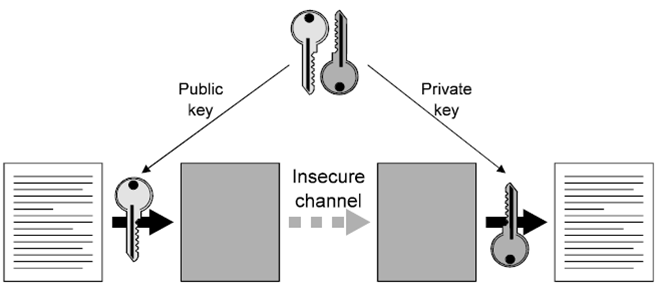
\includegraphics[scale=0.5]{Images/asymg}
\end{figure}
\end{frame}



\begin{frame}{Asymmetric-key cryptography}
\textbf{Data encryption}
\begin{figure}[t]
\centering
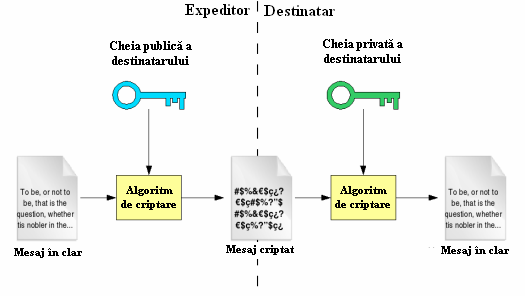
\includegraphics[scale=1]{Images/asyme}
\end{figure}
\end{frame}



\begin{frame}{Asymmetric-key cryptography}
\textbf{Data encryption}
\begin{itemize}
\item
Analogie
\begin{itemize}
\item
Cutia poştală a unei persoane:
\item
Oricine care cunoaşte adresa persoanei respective poate să îi pună o scrisoare în cutie
\item
Numai proprietarul cutiei poştale, care are cheia acesteia, poate să citească scrisorile
\end{itemize}

\item
Pentru criptare şi decriptare se folosesc chei diferite:
\begin{itemize}
\item
Cheia publică a destinatarului la criptare (ea este accesibilă oricui şi deci oricine poate trimite un mesaj unui anumit destinatar)
\item
Cheia privată a destinatarului la decriptare (ea este cunoscută numai de către destinatar şi deci numai acesta poate decripta mesajul)
\end{itemize}
\end{itemize}
\textbf{data confidentiality, data integrity}
\end{frame}



\begin{frame}{Asymmetric-key cryptography}
\textbf{Digital signatures}
\begin{figure}[t]
\centering
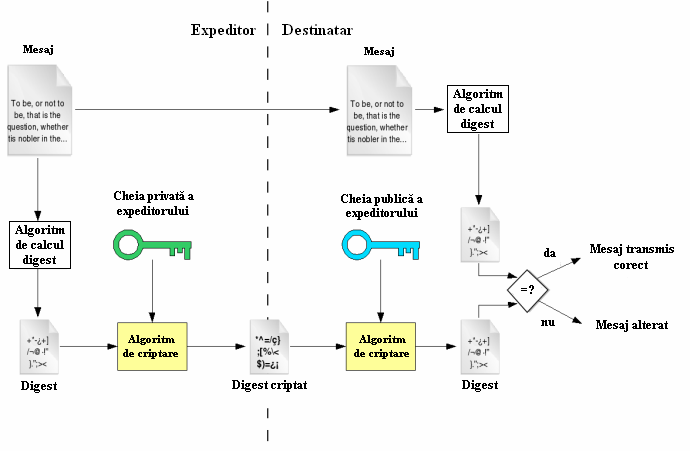
\includegraphics[scale=0.8]{Images/asyms}
\end{figure}
\end{frame}



\begin{frame}{Asymmetric-key cryptography}
\textbf{Digital signatures}
\begin{itemize}
\item
Analogie
\begin{itemize}
\item
Sigilarea unui plic cu un sigiliu de ceară
\item
Oricine poate să deschidă plicul
\item
Numai posesorul sigiliului poate să sigileze plicul
\end{itemize}

\item
Numai expeditorul a putut cripta digestul în forma primită, deoarece cheia privată este cunoscută numai de către el

\item
Oricine poate decripta şi verifica digestul, deoarece cheia publică este accesibilă tuturor
\end{itemize}
\textbf{data integrity, data/origin authentication, data/origin non-repudiation}
\end{frame}



\begin{frame}{Asymmetric-key cryptography}
\textbf{Digital signatures}
\begin{itemize}
\item
Recommended  Key Lengths for electronic signatures:
\begin{itemize}
\item
2048 bits key RSA
\item
2048 bits key DSA
\item
224, 256+ bits Elliptic Curves-based DSA (ECDSA)
\end{itemize}

\item
Un sistem de semnătură digitală implică 3 funcții (algoritmi):
\begin{itemize}
\item
funcția de generare de chei
\item
funcția de semnare
\item
funcția de validare a semnăturii

\end{itemize}
\end{itemize}
\end{frame}



\begin{frame}{Asymmetric-key cryptography}
\textbf{Digital signatures}
\begin{figure}[t]
\centering
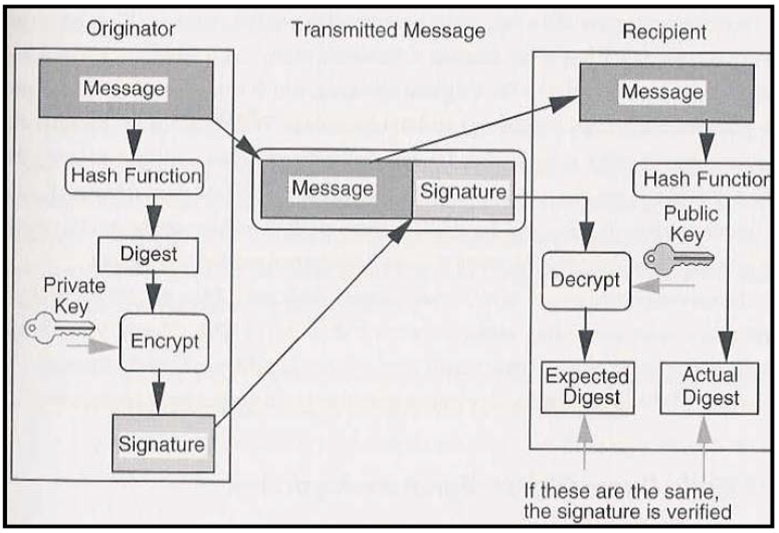
\includegraphics[scale=0.5]{Images/signcs}
\end{figure}
\end{frame}



\begin{frame}{Asymmetric-key cryptography}
\begin{itemize}
\item
Problema centrală a criptografiei cu chei publice:
\begin{itemize}
\item
\textbf{Încrederea} că o anumită cheie publică este:
\begin{itemize}
\item
corectă, 
\item
aparţine persoanei sau entităţii căreia se spune că aparţine 
\item
nu a fost alterată sau modificată de către o terţă parte rău-voitoare
\end{itemize}
\end{itemize}

\item
Soluţii:
\begin{itemize}
\item
prin utilizarea certificatelor:
\begin{itemize}
\item
Web of Trust (folosită de către PGP)
\item
Public-Key Infrastructure (PKI)
\end{itemize}
\item
prin utilizarea identității ca și cheie publică:
\begin{itemize}
\item
Identity-based Cryptography (IBC)
\end{itemize}
\end{itemize}
\end{itemize}
\end{frame}



\begin{frame}{Hybrid cryptography}
\begin{itemize}
\item
Foloseşte pentru criptare atât criptografia simetrică, cât şi cea asimetrică
\item
Avantaje:
\begin{itemize}
\item
Criptografia simetrică este mult mai rapidă decât cea cu chei publice
\item
Gestiunea cheilor în cadrul criptografiei asimetrice este mult mai simplă
\item
Combinarea lor elimină dezavantajul criptografiei simetrice dat de necesitatea de distribuire sigură a cheilor prin criptarea acestora folosind algoritmii asimetrici
\item
Se eliminăşi dezavantajul de viteză al criptografiei asimetrice prin criptarea mesajului propriu-zis folosind algoritmii simetrici
\end{itemize}
\end{itemize}
\end{frame}



\begin{frame}{Hybrid cryptography}
\begin{itemize}
\item
Cum se face defapt criptarea?
\begin{itemize}
\item
Se alege unul din algoritmii de criptare simetrică
\item
Se generează aleator o cheie pentru acest algoritm simetric
\item
Se criptează mesajul folosind algoritmul simetric şi cheia generată
\item
Se criptează cheia simetrică generată folosind cheia publică a destinatarului
\item
Mesajul criptat şi cheia simetrică criptată sunt expediate destinatarului
\item
Destionatarul decriptează cheia simetrică folosind cheia sa privată
\item
Apoi, pe baza cheii simetrice decriptate, decriptează și mesajul propriu-zis
\end{itemize}
\end{itemize}
\end{frame}



\begin{frame}{Hybrid cryptography}
\begin{figure}[t]
\centering
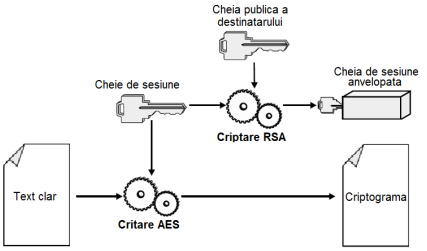
\includegraphics[scale=0.65]{Images/hybrid}
\end{figure}
\end{frame}



\begin{frame}{Hybrid cryptography}
\textbf{Criptarea pentru mai mulți destianatari}
\begin{figure}[t]
\centering
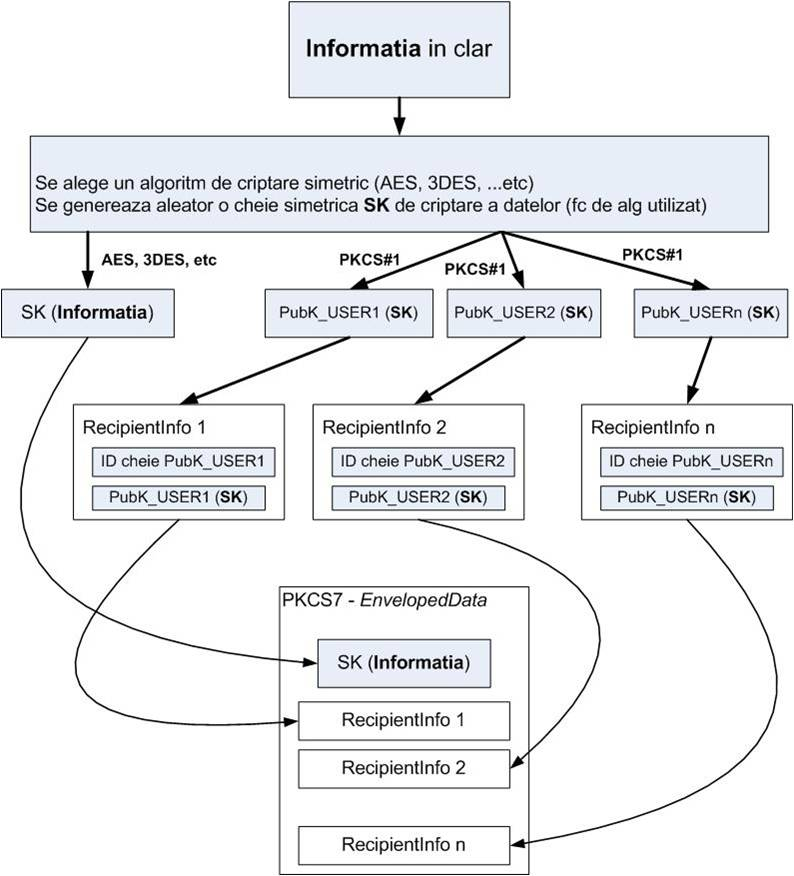
\includegraphics[scale=0.49]{Images/hybridm}
\end{figure}
\end{frame}



\begin{frame}{Key Agreement}
\begin{itemize}
\item
objective: 
\begin{itemize}
\item
key sharing for data encryption \& MACs (data confidentiality, data integrity, data authentication)
\end{itemize}

\item
establishment of the secret keys (key sharing), allows two parties to agree on a shared key

\item
public key-based algorithms: Diffie Hellman, ECDH, RSA

\item
provides part of the required secure channel for exchanging a conventional encryption key

\end{itemize}
\end{frame}



\begin{frame}{Key Agreement}
\begin{figure}[t]
\centering
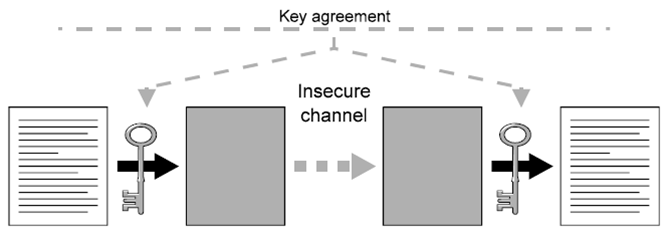
\includegraphics[scale=0.6]{Images/ka}
\end{figure}
\end{frame}



\begin{frame}{Public-Key Cryptography Standards}
\begin{itemize}
\item
PKCS\#1 – std. pt criptografia cu alg. RSA
\item
PKCS\#2 – incorporat in \#1 - criptarea digest–urilor criptografice   
\item
PKCS\#3 – std. Diffie si Hellman Key Agreement
\item
PKCS\#4 – incorporat in \#1 – formatul cheii RSA
\item
PKCS\#5 – std. pt. criptografia bazata pe parole
\item
PKCS\#6 – std. pt. sintaxa extinsa a unui certificat digital – extensii
\item
PKCS\#7 – std. pt. formatul mesajului criptografic
\end{itemize}
\end{frame}



\begin{frame}{Public-Key Cryptography Standards}
\begin{itemize}
\item
PKCS\#8 – std. pt. sintaxa cheii private
\item
PKCS\#9 – std. pt. tipurile de atribute
\item
PKCS\#10 – std. pt. formatul cererii de certificat
\item
PKCS\#11 – std. pt. API–urile criptografice ale dispozitivelor hardware
\item
PKCS\#12 – std. pt. token-uri software 
\item
PKCS\#13 – std. pt. criptografia cu curbe eliptice – in dezvoltare
\item
PKCS\#14 – std. pt. generatoarele de nr. pseudoaleatoare – in dezvoltare
\item
PKCS\#15 – standard pt. formatul informatiei pe token–urile criptografice
\end{itemize}
\end{frame}



\begin{frame}{References}
\begin{itemize}
\item
Alexander Holbreich, Cryptography basics

\url{http://alexander.holbreich.org/cryptography-basics/}

\item
Troy Hunt, Our password hashing has no clothes

\url{https://www.troyhunt.com/our-password-hashing-has-no-clothes/}

%\item


\end{itemize}
\end{frame}



\end{document}